% Crank-002 impact — what the deterministic corrector measurably did to the
% materialized graph. All numbers are read off the Jena graph (//corpus), not
% estimated. Built via rules_tectonic (//impact:needle).
\documentclass[landscape,11pt]{article}

\usepackage[utf8]{inputenc}
\usepackage[T1]{fontenc}
\usepackage[margin=0.7in,landscape]{geometry}
\usepackage{tikz}
\usepackage{pgfplots}
\pgfplotsset{compat=1.18}
\usepackage{microtype}

\definecolor{ratioInk}{HTML}{3A2A1C}
\definecolor{ratioBrown}{HTML}{6E4F34}
\definecolor{ratioTan}{HTML}{B98E5E}
\definecolor{ratioSand}{HTML}{D9C19A}
\definecolor{ratioCream}{HTML}{F4EEDD}
\definecolor{openGreen}{HTML}{2F6B2F}

\pagestyle{empty}
\color{ratioInk}

\begin{document}
\centering

{\Large\bfseries Crank-002 --- the corrector, measured on the graph}\\[2pt]
{\small The deterministic compaction over the materialized ratio corpus. Numbers read from Jena, not estimated.}\\[10pt]

% ---- stat strip ----
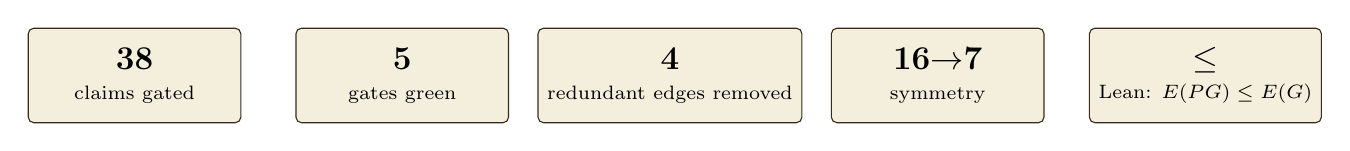
\begin{tikzpicture}
\foreach \x/\val/\lab [count=\i] in {0/38/{claims gated}, 3.4/5/{gates green}, 6.8/4/{redundant edges removed}, 10.2/{16$\to$7}/{symmetry}, 13.6/{$\le$}/{Lean: $E(PG)\le E(G)$}} {
  \node[draw=ratioInk, fill=ratioCream, rounded corners=2pt, minimum width=27mm, minimum height=12mm, align=center] at (\x,0)
    {{\bfseries\large \val}\\[-1pt]{\scriptsize \lab}};
}
\end{tikzpicture}\\[14pt]

\begin{minipage}{0.48\textwidth}
\centering
{\bfseries Deterministic compaction --- same graph, before $\to$ after}\\[4pt]
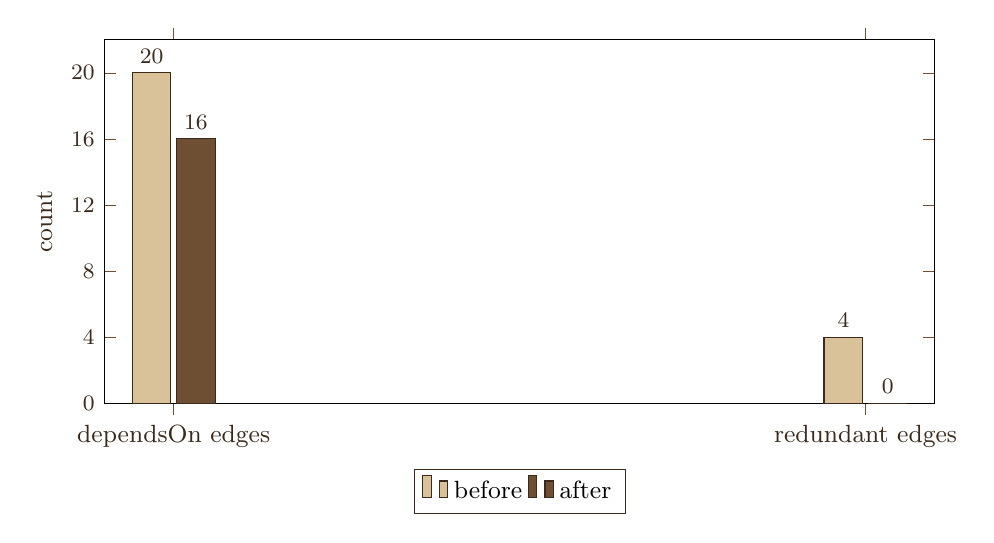
\begin{tikzpicture}
\begin{axis}[
  ybar, bar width=14pt,
  width=\linewidth, height=6.2cm,
  ymin=0, ymax=22,
  symbolic x coords={dependsOn edges, redundant edges},
  xtick=data,
  x tick label style={font=\small\color{ratioInk}},
  ytick={0,4,8,12,16,20},
  ylabel={count}, ylabel style={font=\small\color{ratioInk}},
  y tick label style={font=\footnotesize\color{ratioInk}},
  nodes near coords, nodes near coords style={font=\footnotesize\color{ratioInk}},
  legend style={at={(0.5,-0.18)}, anchor=north, legend columns=2, font=\small, draw=ratioInk},
  tick style={color=ratioBrown},
]
\addplot[draw=ratioInk, fill=ratioSand] coordinates {(dependsOn edges,20) (redundant edges,4)};
\addplot[draw=ratioInk, fill=ratioBrown] coordinates {(dependsOn edges,16) (redundant edges,0)};
\legend{before, after}
\end{axis}
\end{tikzpicture}\\[2pt]
{\scriptsize Transitive reduction: 4 transitively-implied edges dropped (20$\to$16). Closure preserved --- \texttt{:dependsOn} is \texttt{owl:TransitiveProperty}.}
\end{minipage}\hfill
\begin{minipage}{0.48\textwidth}
\centering
{\bfseries Symmetry extracted ($S\!\uparrow$)}\\[4pt]
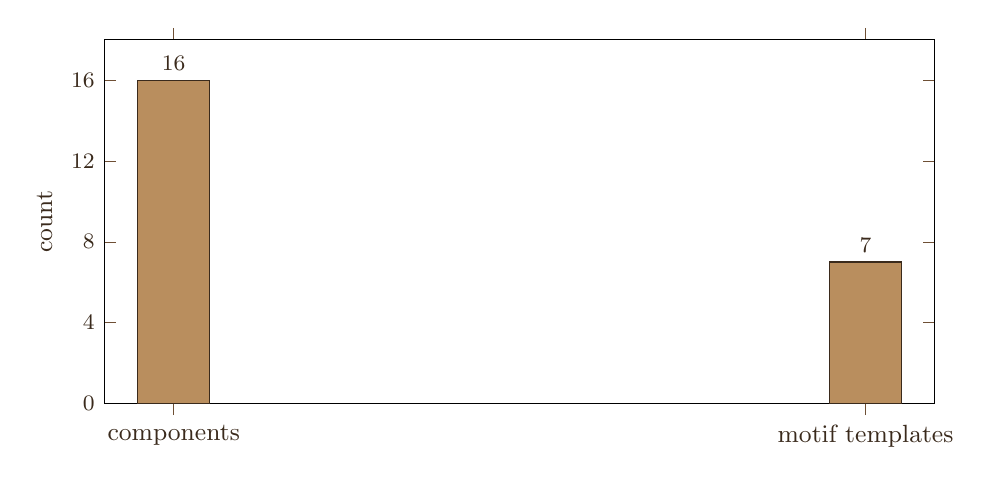
\begin{tikzpicture}
\begin{axis}[
  ybar, bar width=26pt,
  width=\linewidth, height=6.2cm,
  ymin=0, ymax=18,
  symbolic x coords={components, motif templates},
  xtick=data,
  x tick label style={font=\small\color{ratioInk}},
  ytick={0,4,8,12,16},
  ylabel={count}, ylabel style={font=\small\color{ratioInk}},
  y tick label style={font=\footnotesize\color{ratioInk}},
  nodes near coords, nodes near coords style={font=\footnotesize\bfseries\color{ratioInk}},
  tick style={color=ratioBrown},
]
\addplot[draw=ratioInk, fill=ratioTan] coordinates {(components,16) (motif templates,7)};
\end{axis}
\end{tikzpicture}\\[2pt]
{\scriptsize 16 components collapse onto 7 reusable motif templates (M1 the largest orbit at 7). The recoverable symmetry crank-001 estimated, now read from the graph.}
\end{minipage}\\[12pt]

{\footnotesize\color{ratioBrown}
Corrector core proven in Lean (\texttt{//lean:compaction\_test}): meaning-preserving, energy-non-increasing, idempotent --- no \texttt{sorry}. \;
Graph + standard gated green (11/11 tests). \; The corrector only ever lowers $E(G)$.}

\end{document}
